\chapter{Integrating the simulator into Kubernetes}

Batsim is able to run simulations of any distributed system, to study any
event-based scheduler that would implement its message protocol. Kubernetes is
a piece of software where all its component, including the scheduler, revolve
around a central API. Everything is asynchronous as the API can be
accessed anytime by any component.

The question that arises is, can we adapt Batsim to make it support Kubernetes
schedulers? Is it possible to implement an adaptive layer between a synchronous
event based simulator like Batsim and a scheduler implemented following the
asynchronous paradigms of APIs?

It will follow that in order to do so, we re-implemented an API following
Kubernetes specifications and intercepted the scheduler's time to
synchronize it with the simulation time. This allows us to run lengthy
workloads in seconds using a scheduler otherwise supposed to rely on ``real''
machine time. We first describe some technical concepts about Kubernetes and
Batsim, and then describe how we re-implemented the API, intercepted the time,
and handled the synchronization of the different times between Batsim and the
scheduler.


\subsubsection{Batkube features}

TODO: Clearly state what Batkube is capable of, and what it does not do. This
helps describing only the parts of the tools we use while leaving the rest for
the reader to look for on official documentation.

\section{Batsim concepts}

A Batsim simulation is divided into two processes: Batsim itself and the
decision process (the scheduler).  As a consequence, Batsim defines its own
messaging protocol to be able to standardize exchanges with the scheduler. This
protocol takes the form of a text based interface that conveys the events
occuring during the simulation.

\begin{figure}[H]
	\centering
	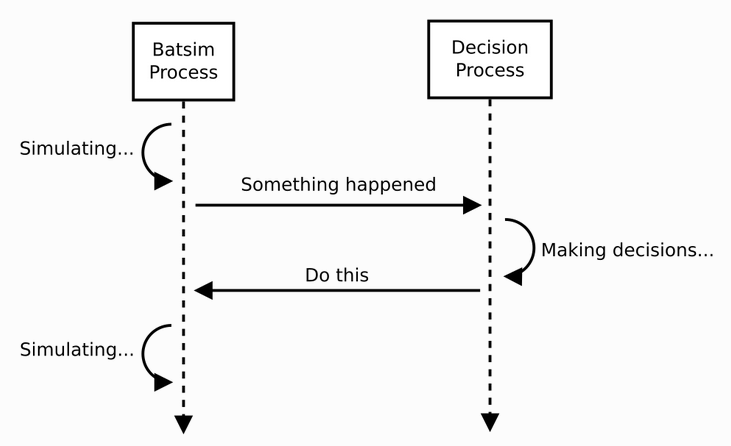
\includegraphics[scale=0.5]{imgs/batsim-sequence-diag.png}
	\captionsource{Exchanges between Batsim and the scheduler.}{https://batsim.readthedocs.io/en/latest/protocol.html}
	\label{fig:bati-seq-diag}
\end{figure}

A Batsim platform is a SimGrid platform, defined in the xml format. A node can
endorse the role of \textit{master}, \textit{compute\_resource} or
\textit{storage}. Here we only consider master nodes which host the decision
process, and compute resources to which we add our custom resource capacities.
These additional fields are \textit{core}\footnote{The core field is already
present in the resource definition, but it is not forwarded to Batsim for
unknown reasons at the time this report is written.} which is the amount of cpu
the node has and \textit{memory} which is memory capacity of the node. Of
course, storage resources can be taken into account in future development of
Batkube. Also, we do not consider the links between the nodes for now because
we do not support parallel jobs. Finally, Batsim proposes an energy model that
we decided to ignore as well.\\

Batsim takes one or several workload as inputs, which are json files containing
jobs definitions. Figure \ref{fig:bat_wl_ex} gives an example of such workload.
The jobs are defined with the following inputs.  First, they are identified by
an \textit{id} which is unique within each workload and are submitted at a time
defined by the \textit{subtime} field. The \textit{res} field states the number
of resources each job requires, although we don't use this field because we
can't specify \textit{which} resource we require. Instead we pass resource
requests as optional parameters. We support the additional fields \textit{cpu}
which has a minimum value of 100m cpu just like Kubernetes cpu
requests\footnote{https://kubernetes.io/docs/concepts/configuration/manage-resources-containers/}
and \textit{memory} which also complies with Kubernetes compute resource
definitions.  Jobs follow a certain \textit{profile} that defines the nature of
the job.  These profile may be as simplistic as \textit{delay} profile which
makes the resource wait for a given amount of time, or describe parallel tasks
using matrices to describe the amount of exchanges between the allocated nodes.
For now we only consider delays to simplify the implementation of the
simulator. Also, because Kubernetes allows the use of multiple
schedulers\footnote{https://kubernetes.io/docs/tasks/extend-kubernetes/configure-multiple-schedulers/},
we support the field \textit{scheduler} which contains the name of the
scheduler the job should be scheduled with.\\

Batsim messaging interface is based on its protocol. Each message is composed
of the field \textit{timestamp} which contains the current simulation time, as
well the field \textit{events} which is a list of events either from Batsim to
the scheduler, or from the scheduler to Batsim. Figure \ref{fig:batmsg_ex}
depicts a standard message sent from the scheduler to Batsim.

Batkube features are limited because we focused on building a working proof
of concept rather than a fully fledged Kubernetes simulator. This is why only
consider a subset of these messages that we present here. More information on
Batsim's protocol is available on Batsim
documentation\footnote{https://batsim.readthedocs.io/en/latest/protocol.html}

TODO: Adrien's view on this section is that it is not necessary and that a link to the doc is sufficient.

\subsubsection{From Batsim to the scheduler}

\paragraph{SIMULATION\_BEGINS}
contains information about the available resources in the cluster, with
Batsim's configuration.

\paragraph{SIMULATION\_ENDS}
is sent at the very end of the simulation: all jobs have finished, and no more
jobs are left in the queues. Batsim exits on this message.

\paragraph{JOB\_SUBMITTED}
notifies the scheduler that a new job has been submitted. It contains
information about the job type, id and specifications. We only consider jobs of
type \textit{delay} to simplify the models. Delay jobs specifications boil down
to the delay length, to which we add resource requests.

\paragraph{JOB\_COMPLETED}
notifies the scheduler that a job has ended, specifying the reason for it. We
only consider situations where all jobs complete correctly. Their state is then
always COMPLETED\_SUCCESSFULLY in our case.

\paragraph{REQUESTED\_CALL}
is an awnser to a CALL\_ME\_LATER event sent by the scheduler.

\subsubsection{From the scheduler to Batsim}

\paragraph{CALL\_ME\_LATER}
is an incentive from the scheduler for Batsim to wake up at a certain
timestamp. When the timestamp is reached in the simulation, Batsim will send a
REQUESTED\_CALL to the scheduler. In our case, this particular exchange will
serve as the base for time synchronisation between the scheduler and Batsim.

\paragraph{EXECUTE\_JOB}
is sent when the scheduler has made a decision. It contains the id of the job
at stake and the id of the resources it has been scheduled to.

\subsubsection{Bidirectional}

\paragraph{NOTIFY}
is used to send some information to the other peer. In our case, we use the
NOTIFY containing no\_more\_static\_job\_to\_submit to determine if the
simulation has ended: knowing that there are no more jobs susceptible to be
scheduled allow us to fast forward to the end of the simulation, thus saving
execution time.\\

Batsim's output takes the form of a csv file containg information about the
jobs executions. Mainly we take interest in their submission time, execution
time and waiting time. Again, a detailed list of Batsim outputs can be found on
the
documentation\footnote{https://batsim.readthedocs.io/en/latest/output-jobs.html}.
During our experimentations with Batkube we interest ourselves in two metrics
that can be computed from this output:
\begin{itemize}
	\item The \textit{makespan}, which is the total length of the
		simulation. It is defined as the timestamp at which the last
		job finishes executing, minus the origin (in this case, zero).
	\item The \textit{mean\_waiting\_time}, which is the mean time the jobs
		spent waiting for a scheduling decision. The waiting time is
		defined by the duration between the submission time and the
		starting time (here the starting time is equivalent to the time
		at which the job was scheduled. We will see later that these
		two times do not correspond in Kubernetes.)
\end{itemize}

These metrics were chosen because in our case, they are representative of the
accuracy of the simulation. Time synchronization (see section
\ref{sec:time-hijack}) may introduce delays in the scheduling decision, thus
increasing the overall makespan and mean waiting time of the simulation.
%Experiments showed that the makespan does not vary much from simulation to
%simulation, but due to Batkube simulations stochastic nature the decisions
%taken by the scheduler may vary from experiment to experiment, thus introducing
%variations in the mean waiting time.

\section{Kubernetes concepts}

Kubernetes is now a large ecosystem to which more than 2 700 developers have
contributed over the years. In this section we present the fundamental concepts
and the components that make up Kubernetes.

\begin{figure}[h]
	\centering
	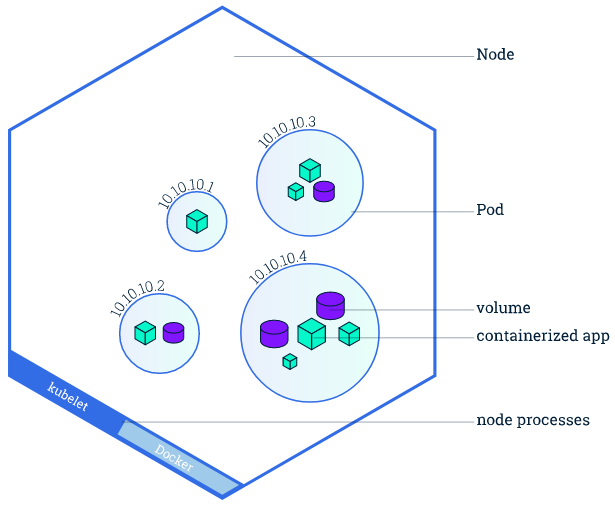
\includegraphics[scale=0.5]{./imgs/node-overview.png}
	\captionsource{Node overview}{https://kubernetes.io/docs/tutorials/kubernetes-basics/explore/explore-intro/}
	\label{fig:node-overview}
\end{figure}

The basic processing unit of Kubernetes is called a \textbf{pod} which is
composed of one or several containers and volumes\footnote{Because of their
	transient nature, containers can not store data on their own. A volume
	is some storage space on the host machine that can be linked to
containers, in order for them to read and write persistent information.}. The
type of application they contain vary depending on the context: in a web
platform context a pod most often hosts a service or micro-service that must be
available at all times, in opposition to a batch processing context where it
runs an application that is to be executed in a finite amount of time.  Pods
are bundled together in \textbf{nodes} (figure \ref{fig:node-overview}) which
are either physical or virtual machines. They represent another barrier to pass
through to access the outside world which bundles pods under the same network
to facilitate communication between them, and enables the use of proxies to
access the underlying services. A set of nodes is called a \textbf{cluster}
which is the highest abstraction layer in Kubernetes.

Nodes take the idea of containerization further than plain containers by
encapsulating the already encapsulated services.  Each node runs at least one
pod, the \textbf{kubelet}, which is a process responsible for communicating
with the rest of Kubernetes. More precisely, the kubelet communicates with the
\textbf{kube-api-server} which is responsible for the whole cluster. We refer
to this API as the api-server, as it is called within the Kubernetes community.
This API server, as well as the other components of the \textbf{Control Plane}
(figure \ref{fig:kube-components}), can be run on any machine but for
simplicity they are set up on the same machine at start up. This machine is
often called the \textbf{master} node and typically does not run any other
container.

As stated before Kubernetes revolves around its API server which is its central
component. All operations between components go through this REST API. These
operations take various forms like user interactions through the commande line
interface \textbf{kubectl}, scheduling operations or management of cluster data
on \textbf{etcd}. We then decided to re-build the API in order to simulate any
cluster to -- almost -- any Kubernetes scheduler.

TODO: Talk about Kubernetes schedulers. What they are based on, how they communicate to Kubernetes.

\begin{figure}[h]
	\centering
	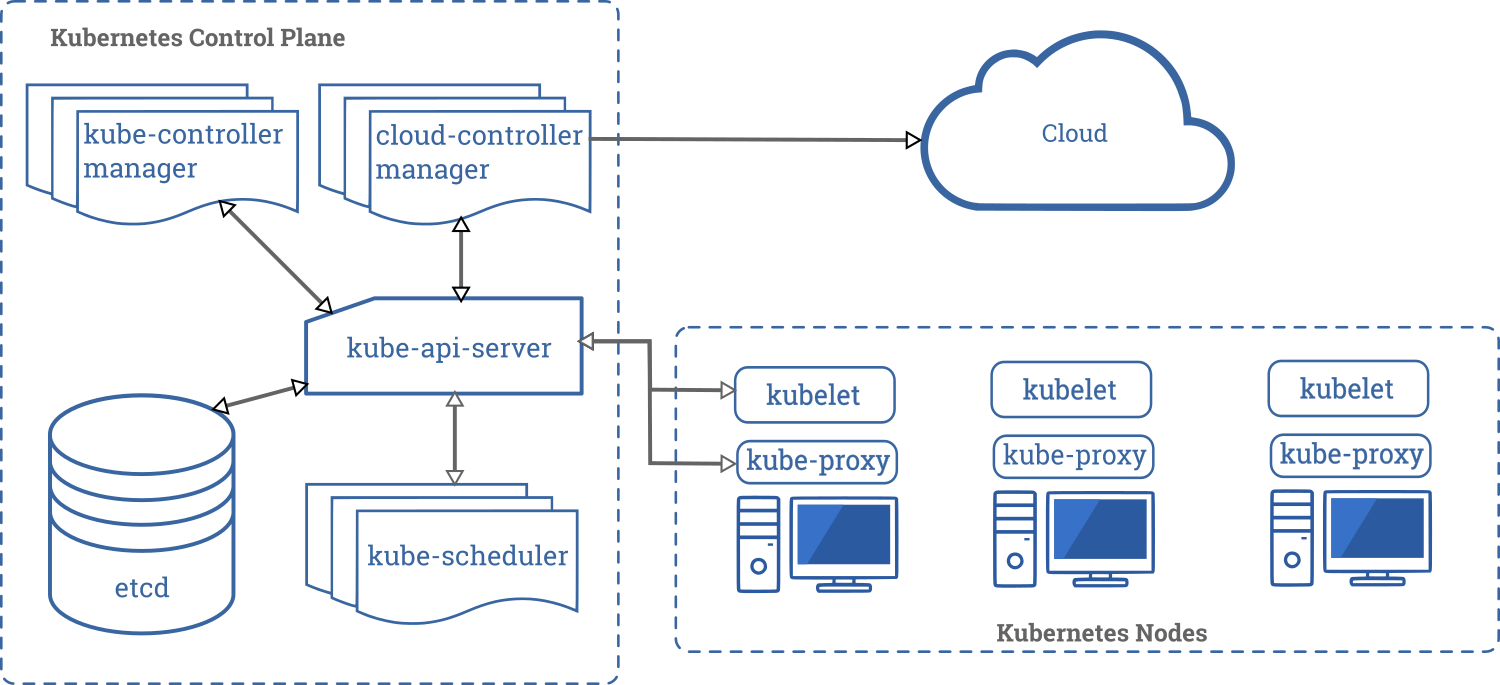
\includegraphics[width=\textwidth]{./imgs/components-of-kubernetes.png}
	\captionsource{Components of Kubernetes}{https://kubernetes.io/docs/concepts/overview/components/}
	\label{fig:kube-components}
\end{figure}

\section{General architecture of Batkube and its integration with Kubernetes and Batsim}

\subsection{Integration with Kubernetes}

In order to adapt Kubernetes schedulers for use with Batsim we need to position
ourselves between the Kubernetes scheduler and the cluster. There are several
options here, at different levels of the cluster. All these are made possible
by the fact that Kubernetes is entirely open source and can be reverse
engineered and modified to suit our needs. First we present the options we
considered but did not choose, and then we explain how we wrote a custom REST
API which acts as a Kubernetes cluster to the scheduler, and as an event based
scheduler to Batsim.

\subsubsection{In between the api and the kubelets}

This is the lowest level option. We position the simulator so as to simulate
just the infrastructure and avoid tampering with Kubernetes resource
management, which is done in their API. This approach would allow us to
effortlessly use any Kubernetes scheduler once their API is supported by
Batkube, and potentially produce the most accurate results. However,
interactions between the kubelets and the API are not documented because the
typical user is not supposed to have to deal with this part of Kubernetes. This
would hinder the development of Batkube because a reverse engineering process
would be required beforehand to understand the intricacies of internal
Kuberenetes exchanges.

\begin{figure}[h]
	\centering
	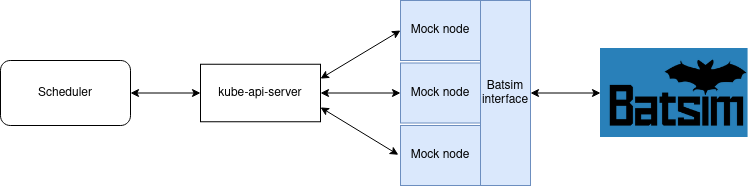
\includegraphics[width=\textwidth]{imgs/architecture-as-kubelets.png}
	\caption{Mocking the cluster itself.}
	\label{fig:mock_nodes}
\end{figure}

\subsubsection{Custom client-go}

Most Kubernetes schedulers rely on
client-go\footnote{https://github.com/kubernetes/client-go}, which is a Go
client for the api-server. It is a library implementing various tools to help
schedulers converse with the API. By altering this client and patching
schedulers so they use our client instead, we can make it exchange with Batsim
instead of the API. 

\begin{figure}[h]
	\centering
	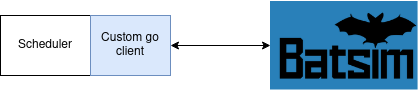
\includegraphics[scale=0.8]{imgs/custom-go-client.png}
	\caption{Custom Go client to redirect scheduler communications to Batsim}
	\label{fig:custom-go-client}
\end{figure}

Contrary to the kubelets, client-go is a user interface and therefore it is
documented, facilitating reverse engineering of its source code. Still, it
represents thousands of lines of code and altering it to our needs would not be
an easy feat.  The other drawback to this approach is that Batkube would only
support schedulers written in Go and making use of client-go, although this
should not be an issue as the only kubernetes scheduler we could find that does
not rely on client-go is a toy scheduler written in bash \cite{bash-scheduler}.

\subsubsection{Custom API}


Re-implementing the API offers a middle ground between the low level and
undocumented solution of the mock nodes, and the higher level and technically
challenging solution of a client-go fork. Again, there are several options here.

A partial reimplementation of the API would save us the task of building a new
API from the ground up. However this would imply digging deep into the
api-server code in order to understand how the api is organized and what code
we would have to alter. In the end, it is easier to simply build a new API,
since there are tools to help us generate it from its specification.

\begin{figure}[h]
	\centering
	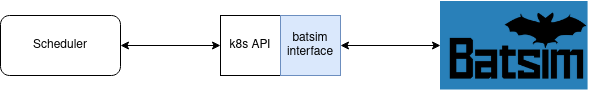
\includegraphics[scale=0.8]{imgs/partial-reimplem.png}
	\caption{Partial reimplementation of the api-server.}
	\label{fig:partial_reimp}
\end{figure}

Furthermore, building a new API allows us to consider only the endpoints we
need and have complete control over the source code. The technically
challenging aspect here is Kubernetes resource management. Indeed, we need to
provide the scheduler with expected informations about the cluster state if we
want to obtain a correct behavior from it, and while the endpoints of the API
are well documented, Kubernetes team did not write lengths about how resources
are managed internally.

\begin{figure}[h]
	\centering
	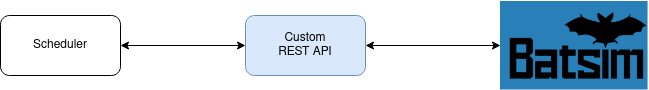
\includegraphics[width=\textwidth]{imgs/custom-restapi.png}
	\caption{Custom REST API in between the scheduler and Batsim.}
	\label{fig:custom-api}
\end{figure}

\subsection{Architecture of Batkube}

Figure \ref{fig:batkube-architecture} depicts the architecture of Batkube,
which is written in Go.  The central component is the \textbf{broker}. It
handles the messages coming from Batsim and the scheduler while ensuring time
synchronization between them. It is responsible for translating and forwarding
messages between Batsim and the scheduler and orchestrates the synchronization
between the two parties.  \textbf{batsky-go} intercepts the calls to Go
\textit{time} library to ensure the scheduler's time is based on the simulation
time instead of machine time. Time requests are forwarded to Batkube which
replies with the current simulation time.  The complete process to ``hijack''
scheduler time is explained in section \ref{sec:time-hijack}. The \textbf{rest
api} is the reimplementation of the Kubernetes api-server. It ensures the
scheduler gets all the necessary information on the cluster state to make its
scheduling decisions, and it is also the receiver of those decisions. Section
\ref{sec:api} explains how we built this API and a tool to automatically
generate its code from the api-server specification.  \textbf{translate} is a
utility package providing functions to translate Kubernetes resources to Batsim
messages, and \textit{vice versa}.

\begin{figure}[h]
	\centering
	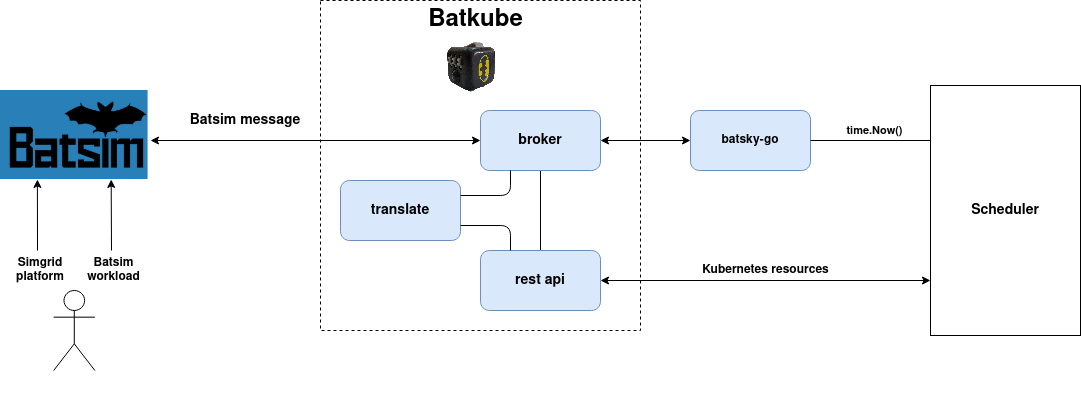
\includegraphics[width=\textwidth]{imgs/batkube-architecture-3-synchro.png}
	\caption{Architecture of Batkube}
	\label{fig:batkube-architecture}
\end{figure}

\section{Building the API} \label{sec:api}

The API of Kubernetes follows the
OpenAPI\footnote{https://www.openapis.org/about} 2 specification which is a
standard for describing APIs. Luckily tools exist to generate such
specification from source code, but also to generate code from a specification.
Since the Kubernetes API specification is available on their
reposotory\footnote{https://github.com/kubernetes/kubernetes/blob/release-1.18/api/openapi-spec/swagger.json},
we were able to use such tools. This allowed us not to implement boiler plate
code by hand and fill the gaps where they needed to be filled, leaving empty
the endpoints we do not need. These endpoints can be dealt with later for
future development of the simulator. For this project we used
go-swagger\footnote{https://github.com/go-swagger/go-swagger/tree/master/examples/stream-server}
to generate our code and the API specification corresponds to the release 1.18
of Kubernetes. One downside of this method is that go-swagger forbids to tamper
with the code of the server itself, although we did not need to during this
project.\\

In order to enable communication between Batsim and the scheduler we need to
translate Batsim messages into Kubernetes resources that can be retrieved by
the scheduler and scheduler decisions to Batsim messages. Batsim Jobs are
simply translated to pods. Jobs do exist in Kubernetes, but they are simply
wrappers around pods: when submitting a job to the (real) api-server, the api
ensures that a pod is created and executed to completion. In our case, we do
not need such intermediate. Compute resources are simply translated to
Kubernetes nodes.

\section{Time interception} \label{sec:time-hijack}

Kubernetes schedulers are not event based schedulers. They constantly check on
the cluster state and make decisions accordingly, therefore they are based on
machine time to make their decisions. However, in order to have correct
simulations, the scheduler needs to be synchronized with simulation time. We
then need to intercept all calls to machine time to redirect them to the
simulator. There are two approaches to this: either we patch the C library used
by Go (figure \ref{fig:patch-C}) and compile Go using our library, or we patch
Go's time library (\ref{fig:patch-Go}) and then patch the scheduler so it uses
our library instead of the official one.

\begin{figure}[]
	\begin{subfigure}{0.5\textwidth}
		\centering
		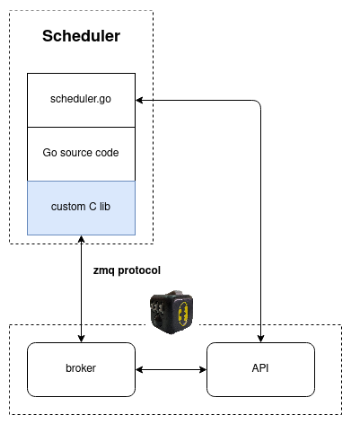
\includegraphics[scale=0.8]{imgs/time-hijack-C.png}
		\caption{Option A: patching the C library}
		\label{fig:patch-C}
	\end{subfigure}
	\begin{subfigure}{0.5\textwidth}
		\centering
		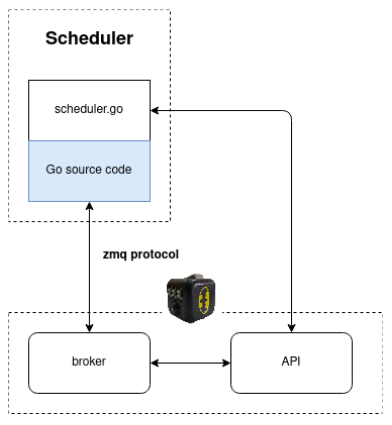
\includegraphics[scale=0.75]{imgs/time-hijack-Go.png}
		\caption{Option B: patching Go}
		\label{fig:patch-go}
	\end{subfigure}
	\caption{Different approaches to intercept the scheduler calls to machine time}
	\label{fig:patch-time}
\end{figure}

An attempt was first made for the custom C library, which is the lowest level
solution. Going for the low level solution would truly redirect all calls to
machine time which is something we can not guarantee with the second option, as
we will see in section \ref{sec:patch-scheds}. This approach proved challenging
due to circular dependency issues and was ultimately abandoned. We opted for
the second option which consist of modifying Go source code, which requires
some additional work to patch the schedulers but was actually easier to
implement.

\subsection{Redirection of time requests to Batkube}

The module in charge of this time redirection is called
\textbf{batsky-go}\footnote{https://github.com/oar-team/batsky-go}, which re
implements \texttt{time.Now()} as well as timers and tickers. Timers are
structures that are instantiated with a duration as input, that notify the
caller once this duration is elapsed. Timers can be reset, modified or deleted
after initialization, which make their implementation tricky in a parallel
computing context. Tickers are essentially the same structures as timers,
except they regularly notify the caller with the given period of time instead
of exiting like timers would.

In order to explain batsky-go algorithms as clearly as possible we need to
provide some context about Go channels, which are structures made for running
code in parallel. Go allows the user to run multi threaded code easily thanks
to its \textbf{go routines}. Whenever in the code the user may create a routine
which will create a new thread and launch the given code parallel to the
encapsulating function. Essentially, this creates a child process.  Go channels
are \textit{``a typed conduit through which you can send and receive values
with the channel operator, <-''}\footnote{source:
https://tour.golang.org/concurrency/2}

\begin{figure}[H]
	\begin{minted}{go}
ch <- v    // Send v to channel ch.
v := <-ch  // Receive from ch, and
           // assign value to v.
   \end{minted}
   \caption{Usage of a Go channel}
   \ref{fig:go-channel}
\end{figure}

\SetKwInput{KwInput}{Input}
\SetKwInput{KwOutput}{Output}

\begin{algorithm}[H]
\DontPrintSemicolon
\KwResult{Current simulation time}
\KwInput{d: timer duration, req: requests channel, res: response channel map}
\KwOutput{now : simulation time}

\If{requester loop is not running}{
	go runRequesterLoop() \tcc{There can only be one loop runing at a time}
}
id = newUUID()\;
m = newRequestMessage(d, id) \tcc{Requests are identified using uuids}
resChannel = newChannel()\;
res[id] = resChannel \tcc{A channel is associated with each request}
req $<$- m \tcc{The code blocks here until request is handled}
now = $<$-resChannel \tcc{The code blocks here until response is sent by the requester loop}
return now\;
\caption{Time request (time.now())}
\label{alg:now}
\end{algorithm}

\begin{algorithm}[H]
\DontPrintSemicolon
\KwInput{req: requests channel, res: response channel map}
\While{Batkube is not ready} {
	wait\;
}
requests = []request\;
\While{req is not empty} {
	m = $<$- req \tcc{Non blocking receive}
	requests = append(requests, m)\;
}
sendToBatkube(requests) \tcc{Only requests with duration > 0 are actually sent. Batkube will always anwser.}
now = responseFromBatkube()\;
\For{m in range requests} {
	res[m.id] $<$-now \tcc{The caller continues execution upon reception}
}

\caption{Requester loop}
\label{alg:reqLoop}
\end{algorithm}



\subsection{Patching schedulers} \label{sec:patch-scheds}

TODO: Explain the AST approach and how it is not a plain sed. (conflict in the
resources used, we have to replace all calls to time's \textbf{functions} and
leave the \textbf{objects} as they are).

\section{Time synchronization}

TODO: explanatory text on this diagram. Explain the different parameters:
timeout, max \& base timestep \& backoff multiplier, min delay, scheduler crash
detection, fast forward on no pending jobs.
\begin{figure}[H]
	\centering
	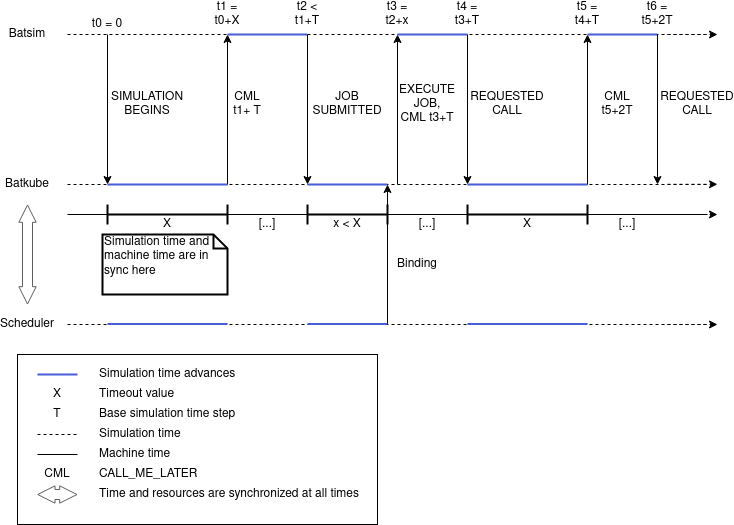
\includegraphics[width=\textwidth]{imgs/lignes_de_temps.png}
	\caption{Time sync between the three components. The broker has to take
	into account both machine time and simulation time.}
	\label{fig:time_sync}
\end{figure}
